\documentclass[final]{dynafront2026}
\usepackage{booktabs}
\usepackage{microtype}

\title[Finite-Rate Selection in Annealed Gibbs Sampling]{A Finite-Rate Selection Law for Annealed Gibbs Sampling}

\optauthor{%
  \Name{Izhar Ali} \Email{aliz@rowan.edu}\\
  \addr Department of Computer Science, Rowan University
  \AND
  \Name{Muhammad Haris Khan} \Email{dcg967@ku.dk}\\
  \addr Department of Computer Science, University of Copenhagen
  \AND
  \Name{Saeed Ahmad} \Email{saeedahmad@iklab.ai}\\
  \addr IKLAB Inc.
}

\newcommand{\qeq}{q_{\mathrm{eq}}}
\newcommand{\qchain}{q_{\mathrm{chain}}}
\DeclareMathOperator{\logit}{logit}

\begin{document}
\maketitle

\begin{abstract}
A sampler can generate plausible examples in the wrong proportions. We show
how this happens in annealed Gibbs sampling, which updates one variable at a
time while lowering the temperature. In the Curie--Weiss model, binary
variables tend to share one sign, giving two modes, and a weak bias, the field, favors one
mode. Each run selects a mode as the modes appear,
when the noise of the updates can still outweigh the field, and rarely switches
afterwards. The samples therefore keep only a fraction of the model's log-odds
between the modes. We turn the classical probability of this selection, due
to Kondepudi and Nelson, into a law for this fraction. The law agrees closely with
an exact calculation of the sampler and explains why slower cooling
helps little: on a linear ramp, cooling sixteen times more slowly only doubles
the fraction. In a Hopfield model, competition among stored patterns raises
the fraction. On one linear ramp, we predict the fraction as the exact Curie--Weiss fraction times a
competition factor derived under a Gaussian approximation. This pre-registered prediction is within 3\% of the measured fraction for three
patterns at three sizes; for four patterns, the measurement is 6\% lower.\footnote{Code and details:
\url{https://github.com/ali-izhar/finite-rate-selection-law}}
\end{abstract}

\section{Introduction}
\label{sec:intro}

Suppose a model of handwritten digits assigns twice as much probability to
``3'' as to ``8''. A sampler should then produce about twice as many ``3''s as
``8''s over many runs. It can produce recognizable examples of both digits and
still get this proportion wrong, and Monte Carlo estimates from its samples are
then biased. How does the sampler change these proportions?

We study annealed Gibbs sampling, which redraws one variable at a time from its
conditional distribution. At high temperature the
model's distribution is broad; at low temperature its probability concentrates in
modes, regions of likely outcomes separated by unlikely ones. As the
temperature falls, the regions between modes become even less likely and the sampler stops mixing between them: later updates mostly sharpen the
mode each run selected and rarely undo the selection \citep{neal2001}.

The sampler can therefore get the mode proportions wrong even when the model
is right. To measure this error alone, we use the Curie--Weiss (CW) model, whose
probabilities, and its Gibbs sampler's, can be computed exactly. Its binary
variables tend to align, giving two modes below a critical temperature: most variables positive,
or most negative. A weak field, a bias on every variable, favors the positive
mode, but each run selects its mode near the critical temperature, where the noise
of the Gibbs updates can outweigh the field.

We turn the classical probability of selecting the positive mode, due to
\citet{kondepudinelson1983} \citep[see also][]{kondepudigao1987,nene2018}, into a \emph{selection law}
for the fraction of the model's log-odds between the modes that the samples keep,
and show why slower cooling helps little.
Extended to a Hopfield model, whose modes are stored patterns
and their negatives, the argument predicts that competition among patterns multiplies
the exact CW fraction by a factor that grows with their number.
A pre-registered test on one linear cooling ramp agrees to within $3\%$ for
three patterns at three sizes; for four patterns, the measurement is $6\%$
lower than predicted.

\section{An exact model of mode selection}
\label{sec:model}

The model's state, or \emph{configuration}, is a vector $x=(x_1,\ldots,x_N)$
of $N$ binary variables $x_i\in\{-1,+1\}$, called spins. The CW model gives
higher probability to configurations whose spins agree:
\begin{equation}
 \pi_{\beta,G}(x)\propto
 \exp\!\left[\frac{\beta}{2(N-1)}\sum_{i\ne j}x_i x_j
              +\beta G\sum_i x_i\right].
 \label{eq:model}
\end{equation}
The \emph{inverse temperature} $\beta$ sets how strongly spins prefer to
agree: at $\beta=0$ all configurations are equally likely, and increasing
$\beta$, which is cooling, concentrates probability on aligned
configurations. The field $G$ is fixed during a run and favors positive spins when $G>0$.
At fixed $\beta$, the Gibbs sampler converges to the \emph{equilibrium distribution} $\pi_{\beta,G}$.
The \emph{magnetization} $m=N^{-1}\sum_i x_i$ summarizes a configuration:
$m>0$ means mostly positive spins, $m<0$ mostly negative. Without a field, as
$N\to\infty$, the equilibrium $m$ concentrates at $0$ for $\beta<1$ and at two
opposite nonzero values for $\beta>1$. Configurations with $m$ near either value form
the two modes, and $\beta=1$ marks the \emph{transition}, at the
critical temperature.

A run starts at some $\beta<1$, from the equilibrium distribution at that or a lower $\beta$. Each Gibbs update redraws one uniformly chosen
spin; updates occur at random times, $N$ per unit time on average, and this
unit is an \emph{expected sweep}. A cooling schedule raises $\beta$ past the
transition to a final value, by which the run has settled into one mode. At a given $\beta$, configurations with
the same number $k$ of positive spins are equally probable in equilibrium and change $k$ at the same
rates, which lets $k$, and so $m=2k/N-1$, alone describe the run: we track $N+1$ probabilities, one for each
$k=0,\ldots,N$, instead of $2^N$, one for each configuration
\citep{levinluczak2010}. We compute them exactly, without sampling error, by numerically
solving the linear equations that govern their change (Appendix~\ref{app:exact}).

Each run's final configuration is its sample. Let $\qchain$ be the probability that a sample has $m>0$, and $\qeq$ the
probability of $m>0$ under the equilibrium distribution at the final $\beta$, both
conditioned on $m\ne0$. The fraction of the model's log-odds, $\logit\qeq$, that the samples
keep is
\begin{equation}
 c=\frac{\logit\qchain}{\logit\qeq},
 \qquad \logit q=\log\frac{q}{1-q},
 \label{eq:c}
\end{equation}
for $\qeq\ne1/2$: $c=1$ reproduces the equilibrium proportions, and $c=0$
gives equal mode probabilities. If equilibrium odds are $4{:}1$, $c=0.2$
gives sampled odds of $4^{0.2}{:}1\approx1.32{:}1$.

\section{The selection law}
\label{sec:law}

Each run selects its mode in a short window near $\beta=1$. There, a small random imbalance
between positive and negative spins grows into one mode
(Figure~\ref{fig:mechanism}a); afterwards, switching between modes takes far
longer than settling within one
\citep{levinluczak2010,dlpcmp2009}. The final proportions are therefore
decided in this window, the only time the field can bias them.

\begin{figure}
 \centering
 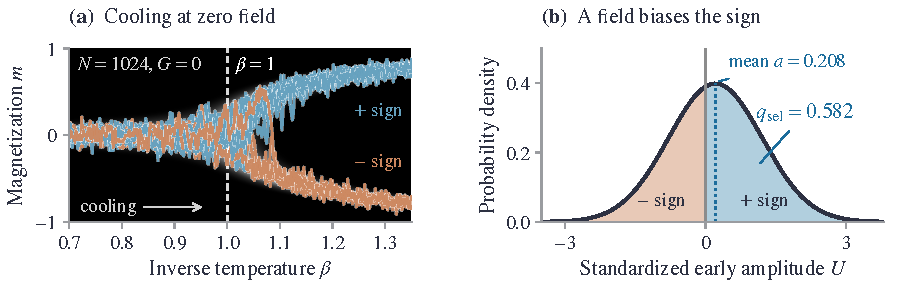
\includegraphics[width=\textwidth]{figures/mechanism}
 \caption{
 (a) Fourteen paths ($N=1024$, $G=0$) of $m$ under the drift
 $-m+\tanh(\beta m)$ plus Gaussian noise, approximating the Gibbs chain, split into two modes; the dashed curves mark the most probable equilibrium magnetization. (b) Analytical density of the standardized early amplitude
 $U\sim\mathcal N(a,1)$ on a linear ramp ($N=2048$, $\gamma=0.001$, $G=0.0006125$).}
 \label{fig:mechanism}
\end{figure}

Near the transition, two effects move $m$ (Appendix~\ref{app:exact}). The \emph{drift}, the mean rate of change of $m$, is
$-m+\tanh(\beta m+\beta G)$, approximately \mbox{$(\beta-1)m+G$} near $m=0$
and $\beta=1$. Below $\beta=1$ the term $(\beta-1)m$ points against $m$ and pulls an
imbalance back toward zero; above $\beta=1$ it points along $m$ and amplifies
the imbalance. The \emph{noise} comes from the randomness of the Gibbs updates
and adds a variance of about $2/N$ per expected sweep. On a linear ramp at cooling rate $\gamma>0$,
$\beta(t)=1+\gamma t$ crosses $\beta=1$ at $t=0$. The growth rate $\beta-1=\gamma t$
then rises with time, and the drift multiplies the imbalance by
$e^{\gamma t^2/2}$, a factor that stays near one only for $|t|$ below a time $T$ of order
$\gamma^{-1/2}$: this is the window. Within it, the field adds an imbalance of
order $GT$ and the noise one of order $\sqrt{T/N}$ \citep{berglundgentz2002}.
Their ratio, of order $G\sqrt N\,\gamma^{-1/4}$, decides whether the field or the noise sets the sign: slower
cooling widens the window and favors the field, but only as $\gamma^{-1/4}$.

To turn the field-to-noise ratio into the probability that a run ends in the
positive mode, we divide $m$ by its growth factor $e^{\gamma t^2/2}$.
The result, the early \emph{amplitude}, has the sign of $m$ and stops
changing once the window closes, because later kicks are divided by a large growth factor. It is the field's push, the same in every run,
plus the accumulated noise, a sum of independent Gaussian kicks; in
the linear approximation it is therefore Gaussian across runs, with mean set
by the field and spread by the noise. In units of its spread, it follows $U\sim\mathcal N(a,1)$,
where $a$ is this field-to-noise ratio with its exact prefactor. In the linear approximation, a
run ends with $m>0$ when $U>0$, which happens with probability
$\Phi(a)$ (the blue area in Figure~\ref{fig:mechanism}b), where $\Phi$ is the
standard Gaussian CDF. For the parameters of Figure~\ref{fig:mechanism}b,
$a=0.208$: the noise is about five times stronger than the
field, yet $58\%$ of runs end in the favored mode. This is the classical result
\citep[][Appendix~\ref{app:exact}]{kondepudinelson1983,kondepudigao1987}
\begin{equation}
 q_{\mathrm{sel}}\simeq\Phi(a),\qquad a=G\sqrt N(\pi/\gamma)^{1/4},
 \label{eq:law}
\end{equation}
with $q_{\mathrm{sel}}$ the probability of selecting $m>0$. Without later switching,
$\qchain=q_{\mathrm{sel}}$.

With $q_{\mathrm{sel}}$ for $\qchain$, Eq.~\eqref{eq:c} gives the \emph{selection
law}, $c_{\mathrm{sel}}=\logit\Phi(a)/\logit\qeq$. For a weak
field ($|a|\ll1$), the sampled log-odds are $\logit\Phi(a)\approx4a/\sqrt{2\pi}$,
proportional to $a$, hence to $G\sqrt N\,\gamma^{-1/4}$. The equilibrium
log-odds at the final temperature grow faster with $N$, as $NG$, than the sampled log-odds: reversing all $N$
spins leaves the coupling term unchanged and reverses the field term, $\beta GNm$, of order $NG$ in either mode. In their
ratio, the field cancels, and $c$ measures the sampler, not the field
(prefactor: Appendix~\ref{app:exact}):
\begin{equation}
 c\propto(N^2\gamma)^{-1/4}.
 \label{eq:scaling}
\end{equation}
For a weak field, cooling sixteen times more slowly doubles $c$; a fourfold
larger $N$ halves it.

The selection law rests on four assumptions (Appendix~\ref{app:exact}): a slow ramp
($\gamma\ll1$), a start well below $\beta=1$, a nearly linear drift, and little switching
after selection. For bounded $a$, $N\gamma\gg1$ guarantees the third \citep{berglundgentz2002}:
the noise gathered in the window is then a fraction $(N\gamma)^{-1/2}$ of the magnitude
$|m|\sim\gamma^{1/4}$ at which the drift turns nonlinear. Very slow cooling violates the last, since long
enough sampling restores the equilibrium proportions; but at $N=2048$ and $\beta=1.1$, a
zero-field switch between modes takes on average about $5\times10^{7}$ expected sweeps (the exact chain's mean passage time); our
ramps last at most $3600$ expected sweeps.

\paragraph{Exact check.}
On linear ramps ($N=1024$--$4096$, $\gamma=0.00025$--$0.004$,
$NG=1.2544$), exact $c$ exceeds $c_{\mathrm{sel}}$ by $0.23$--$1.81\%$ (Figure~\ref{fig:validation}a; Appendix Table~\ref{tab:linear}), even
at $N\gamma=0.256$, where $N\gamma\gg1$ fails.

\begin{figure}
 \centering
 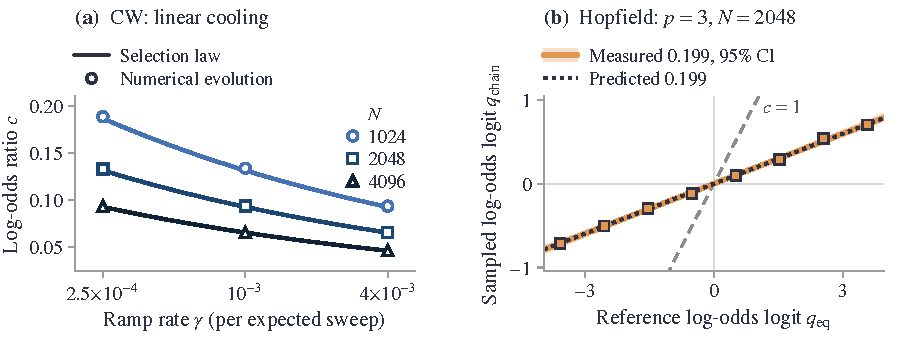
\includegraphics[width=\textwidth]{figures/validation}
 \caption{(a) CW ramps at fixed $NG$: the law is within $2\%$.
 (b) Hopfield: ratio of measured to predicted $c$ for the eight rows of
 Table~\ref{tab:transfer}, with the predictions of Section~\ref{sec:test}; bars are $95\%$ intervals.}
 \label{fig:validation}
\end{figure}

\section{When several modes compete}
\label{sec:test}

CW has two modes. To ask how competition among several modes changes the
fraction $c$, we use the Hopfield model: with $p\ll N$ stored patterns
$\xi^\mu\in\{-1,+1\}^N$ of independent equiprobable entries, its
modes at low temperature are the patterns and their negatives
\citep{ags1985}. A configuration $x$ has probability proportional to
$e^{-\beta E_G(x)}$, with \emph{energy}
\begin{equation}
 E_G(x)=-\frac{1}{2(N-1)}\sum_{i\ne j}\sum_{\mu=1}^p
       \xi_i^\mu\xi_j^\mu x_i x_j-G\sum_i\xi_i^1x_i.
 \label{eq:hopfield}
\end{equation}
The field $G$ favors pattern~1 over its negative. The overlap $m^\mu=N^{-1}\sum_i\xi_i^\mu x_i$ measures
how closely a configuration resembles pattern $\mu$: it is $+1$ at pattern $\mu$ and $-1$ at its negative.
For $p=1$, the variables $y_i=\xi_i^1x_i$ turn $e^{-\beta E_G}$ into Eq.~\eqref{eq:model} and $m^1$ into
the magnetization of $y$: the CW model is the one-pattern Hopfield model. Because the map is one to
one and acts spin by spin, it also turns each Gibbs update of $x$ into one of $y$, so a one-pattern
run is a CW run (Appendix~\ref{app:protocol}). Each
sample is labeled by the pattern with the largest $|m^\mu|$ and the
sign of that overlap. Here $\qchain$ and $\qeq$ are the probabilities that a pattern-1
sample has the positive sign, so $c$ compares log-odds of that sign, not pattern frequencies.

Competition raises the fraction. We assume that the overlaps' early amplitudes
(Section~\ref{sec:law}) are independent Gaussians of common variance;
that the field shifts only the mean of pattern~1's; and that a run ends in the
pattern whose early amplitude is largest in magnitude. Pattern~1's sign log-odds
at amplitude magnitude $r$ then equal the log ratio of a shifted
Gaussian's densities at $+r$ and $-r$, which is linear in $r$. Winning depends only on
magnitude and leaves these log-odds unchanged at each $r$, but the winner of $p$ amplitudes has a larger
average magnitude than a single one; to first order in the
field, its sign log-odds are multiplied by the ratio of the two average magnitudes:
\begin{equation}
 A_p=\frac{\mathbb E\max_{1\le\mu\le p}|Z_\mu|}{\mathbb E|Z|},
 \qquad c_{\mathrm{pred}}=A_p c_{\mathrm{CW}},
 \label{eq:amplification}
\end{equation}
where $Z$ and the $Z_\mu$ are independent standard Gaussians: $|Z_\mu|$ is the
size of pattern $\mu$'s early amplitude in units of its spread; the denominator is the average size of a single amplitude, as in CW, where the one pattern always wins.
Here $c_{\mathrm{CW}}$ is the exact CW fraction on the test's ramp (below), not the selection law's value, so
the test below checks Eq.~\eqref{eq:amplification}, not the selection law.
Appendix~\ref{app:amplification} derives Eq.~\eqref{eq:amplification};
numerical integration gives $A_1=1$, $A_2=\sqrt2$,
$A_3=1.662$, and $A_4=1.836$.

\begin{table}
 \centering
 \caption{Pre-registered Hopfield test on one linear ramp ($\gamma=0.004$, $\beta=0.7$ to $1.6$).
 Predictions are the exact chain for $p=1$, the exact two-block value for $p=2$, and $A_pc_{\mathrm{CW}}$ for $p\ge3$. Ratio: measured over predicted $c$. Intervals are $95\%$ and
 resample the $50$ pattern sets.}
 \label{tab:transfer}
 \begin{tabular}{rrlrlr}
 \toprule
 $p$ & $N$ & prediction & predicted $c$ & measured $c$ & ratio\\
 \midrule
 1 & 1024 & exact chain & 0.0937 & $0.0928\ [0.0909,0.0947]$ & 0.990\\
 1 & 2048 & exact chain & 0.0659 & $0.0659\ [0.0647,0.0672]$ & 1.001\\
 1 & 4096 & exact chain & 0.0464 & $0.0472\ [0.0464,0.0480]$ & 1.015\\
 2 & 2048 & exact two-block & 0.0936 & $0.0946\ [0.0928,0.0965]$ & 1.011\\
 3 & 1024 & $A_3c_{\mathrm{CW}}$ & 0.1558 & $0.1518\ [0.1463,0.1571]$ & 0.975\\
 3 & 2048 & $A_3c_{\mathrm{CW}}$ & 0.1095 & $0.1090\ [0.1059,0.1123]$ & 0.995\\
 3 & 4096 & $A_3c_{\mathrm{CW}}$ & 0.0772 & $0.0758\ [0.0734,0.0782]$ & 0.982\\
 4 & 2048 & $A_4c_{\mathrm{CW}}$ & 0.1209 & $0.1137\ [0.1069,0.1210]$ & 0.940\\
 \bottomrule
 \end{tabular}
\end{table}

For two patterns, the prediction needs no Gaussian assumption. In the variables
$y_i=\xi_i^1x_i$, the spins where the two patterns agree and those where they differ form
two CW models that do not interact, and pattern~1 wins exactly when their magnetizations
share a sign (Appendix~\ref{app:amplification}). The exact chain of each block then gives
$c_{\mathrm{pred}}$ for each pattern set; $A_2c_{\mathrm{CW}}$ lies $0.5\%$ below it.

\paragraph{Pre-registered test.}
All runs cool on the fastest ramp of the exact check, where $N\gamma$ is largest, from
$\beta=0.7$ to $1.6$ at $\gamma=0.004$. Runs start from independent unbiased spins, the equilibrium at $\beta=0$, and each update redraws one uniformly chosen spin, as in Section~\ref{sec:model}. Half the runs have
field $+|G|$, half $-|G|$, with $NG=1.2544$, and each row uses
$50$ pattern sets, independent draws of the $p$ patterns. The measured $c$ is the log-odds that a pattern-1 sample takes the
field's sign, pooled over sets and signs, divided by the exact CW $\logit\qeq$; $95\%$
intervals resample pattern sets. This denominator cancels in the ratio of measured to predicted $c$;
it equals the Hopfield $\logit\qeq$ at $p=1$ and is within $1.3\%$ of it where we computed both ($p=2$ at $N=2048$; $p=3$ at $N\le1024$). We fixed the predictions, run counts and readings of the outcome
in advance (Appendix~\ref{app:protocol}).

\paragraph{Result.}
The one-pattern runs reproduce the exact chain at three sizes (ratios $0.990$--$1.015$), which
checks the sampler and the estimator, and the two-pattern runs match the exact two-block value to within $1.1\%$
(Table~\ref{tab:transfer}; Figure~\ref{fig:validation}b). For three patterns at $N=2048$, measured
$c$ is $0.995$ times $A_3c_{\mathrm{CW}}$ ($95\%$ interval $[0.967,1.026]$); at $N=1024$ and $4096$
the ratios are $0.975$ and $0.982$, and their intervals also contain $1$. Over these sizes,
three-pattern $c$ falls as $N^{-0.50}$ (exponent interval $[0.47,0.53]$), as the exact CW fraction
does and as Eq.~\eqref{eq:scaling} predicts at a fixed rate.

\section{Where the competition prediction falls short}
\label{sec:limits}

For four patterns, measured $c$ is $6\%$ below $A_4c_{\mathrm{CW}}$; the interval of their
ratio, $[0.884,1.001]$, contains $1$, but only just. All four $A_pc_{\mathrm{CW}}$ rows lie below
their predictions, by $0.5$--$6\%$. Equation~\eqref{eq:amplification} assumes independent amplitudes
of common variance, but random patterns are correlated: two of them agree on a fraction of spins
that differs from one half by order $N^{-1/2}$. Overlap components along the eigenvectors of the pattern correlation matrix then begin to grow at
slightly different $\beta$, and this spread is small next to the selection window only when
$N\gamma\gg p$ (Appendix~\ref{app:amplification}). Here $p/(N\gamma)$ ranges from $0.18$ to
$0.73$, so no row has $N\gamma\gg p$; a linearized Gaussian model of these components, which we did not validate, gives deficits of $0.5$--$3\%$. The deficits do not follow $p/(N\gamma)$ closely: the largest is at $p=4$,
$N=2048$, not at $p=3$, $N=1024$, where $p/(N\gamma)$ is largest. These differences lie within the intervals, so the rows neither support nor rule out this explanation
(Appendix~\ref{app:protocol}).

The test uses one cooling rate and one value of $NG$, in the
weak-field regime where log-odds are linear in the field, so it does not show how
competition depends on the cooling rate. The selection law and
Eq.~\eqref{eq:amplification} describe single-spin Gibbs sampling; other samplers
need their own calculation.

\section{Discussion}
\label{sec:discussion}

The selection probability is classical
\citep{kondepudinelson1983,kondepudigao1987}; we turn it into the selection
law for $c$, check the law against the exact CW calculation, and extend it to competing
modes. Cooling studies of spin chains \citep{suzuki2009} measure
misaligned regions and excess energy, not mode probabilities.

Annealed importance sampling weights annealed runs to estimate equilibrium
averages \citep{neal2001}; unweighted runs keep only a
fraction $c$. Comparing them at equal cost needs the weighted estimator's bias and
variance. Diffusion models change their distribution gradually, but with an exact
score they reverse a noising process without equilibrating at each step
\citep{biroli2024}; extending our calculation needs their reverse dynamics
and time discretization.
A variance-preserving noise schedule can miss unequal mode probabilities, while suitable
schedules recover them in Gaussian mixtures and CW
\citep{aranguri2025}.

The exact CW calculation gives, without sampling, the mode-probability
error of any cooling schedule; applying $c$ to other models requires
their equilibrium log-odds. Repeating the four-pattern test at several cooling rates would
test the correlation argument, which expects the deficit to shrink as $N\gamma/p$ grows.

\label{main-text-end}
\bibliography{references}

\clearpage
\appendix

\section{Selection law and exact-chain calculations}
\label{app:exact}

This appendix derives the selection law of Section~\ref{sec:law}, states when
it holds, and describes the exact calculation that tests it.

\paragraph{From spin updates to drift and noise.}
The drift and noise of Section~\ref{sec:law} follow from single-spin updates. For a chosen spin, let $\ell_i=\beta(N-1)^{-1}\sum_{j\ne i}x_j+h$,
where $h=\beta G$. Holding the other spins fixed, Eq.~\eqref{eq:model}
assigns weights $e^{\ell_i}$ and $e^{-\ell_i}$ to its two values, so the
redrawn spin has mean $\tanh\ell_i$. For large $N$, the neighbors' average is approximately $m$.
A uniformly chosen spin has old mean $m$, so one update changes $m$ by
$[\tanh(\beta m+h)-m]/N$ in expectation. With $N$ updates per expected sweep,
the drift is $\dot m=-m+\tanh(\beta m+h)$.
Near $m=0$ and in a weak field, an update flips a spin with probability about
one half, and each flip changes $m$ by $2/N$. The noise variance per expected sweep
is therefore approximately $N\times\tfrac12\times(2/N)^2=2/N$.
A short interval contains many updates that change $m$ little; we
approximate the centered sum of their jumps by a Gaussian.
For small $m$ and $G$ near $\beta=1$, we expand $\tanh z=z-z^3/3+\cdots$,
keep the field, linear, and cubic terms, and write $G$ for $h=\beta G$
(equal at $\beta=1$). This gives
\begin{equation}
 dm=\big[(\beta-1)m-m^3/3+G\big]dt+\sqrt{2/N}\,dW_t,
 \label{eq:sde}
\end{equation}
where $W_t$ is a standard Brownian motion.
At $G=0$ and with $\beta$ ramped through $1$, Eq.~\eqref{eq:sde} is the
dynamic pitchfork bifurcation with additive noise analyzed by
\citet{berglundgentz2002}: the drift's single stable value, $m=0$, splits into two.
The paths of Figure~\ref{fig:mechanism}a integrate the drift $-m+\tanh(\beta m)$ with noise
variance $2/N$ per expected sweep by Euler steps of $0.02$, from $m=0$, holding each of $360$
equally spaced values of $\beta$ from $0.7$ to $1.35$ for $6$ sweeps (NumPy seed $4$).

\paragraph{Removing growth without changing the sign.}
On a linear ramp, $\beta-1=\gamma t$. While $m$ is small, omit the cubic
term. Without field or noise, $\dot m=\gamma t m$ has the positive growth
factor $e^{\gamma t^2/2}$. Dividing it out gives $Y_t=e^{-\gamma t^2/2}m_t$,
which keeps the sign of $m_t$; its limit is the early amplitude of Section~\ref{sec:law}. Start at
$t_0<0$. The product rule gives
\[
 Y_t=e^{-\gamma t_0^2/2}m_{t_0}
       +G\int_{t_0}^t e^{-\gamma u^2/2}\,du
       +\sqrt{2/N}\int_{t_0}^t e^{-\gamma u^2/2}\,dW_u.
\]
The three terms are the remaining initial imbalance, the accumulated field,
and the accumulated noise. With $w(u)=e^{-\gamma u^2/2}$, the noise integral
is the limit of sums $\sum_j w(u_j)\sqrt{\Delta u}\,\epsilon_j$ of independent
standard Gaussians $\epsilon_j$: a Gaussian with mean zero and variance
$\sum_j w(u_j)^2\Delta u$.

The weights are appreciable over times of order $\gamma^{-1/2}$ around
the transition. A start well below $\beta=1$ ($|t_0|\gg\gamma^{-1/2}$)
makes the factor $e^{-\gamma t_0^2/2}$ of the initial term negligible; a late end
lets both integrals settle. Extending their limits to the whole real line
gives the early amplitude $Y$ with
\begin{align*}
 \mu_Y=\mathbb E Y
 &=G\int_{-\infty}^{\infty}e^{-\gamma u^2/2}\,du
   =G\sqrt{2\pi/\gamma},\\
 V_Y=\operatorname{Var}(Y)
 &=\frac2N\int_{-\infty}^{\infty}e^{-\gamma u^2}\,du
   =\frac2N\sqrt{\pi/\gamma}.
\end{align*}
Hence $U=Y/\sqrt{V_Y}=a+Z$, where $Z\sim\mathcal N(0,1)$ and
$a=\mu_Y/\sqrt{V_Y}=G\sqrt N(\pi/\gamma)^{1/4}$.
The positive mode is selected when $U>0$, with probability
$\Pr(Z>-a)=\Phi(a)$, as in Eq.~\eqref{eq:law}.
These infinite limits approximate a finite cooling interval; the integrals must settle before the cubic term
substantially changes the amplitude.

\paragraph{From a sign probability to the fraction $c$.}
Eq.~\eqref{eq:c} then turns $\Phi(a)$ into $c$. For small $a$, $\Phi(a)=1/2+a/\sqrt{2\pi}+O(a^3)$.
The derivative of $\logit q$ at $q=1/2$ is $4$, so
$\logit\Phi(a)=4a/\sqrt{2\pi}+O(a^3)$.
At the final inverse temperature $\beta_f$, a field adds $\beta_f NGm$
to each configuration's log weight. Let $\bar m_f$ be the zero-field
mean magnetization in the positive mode at $\beta_f$. To first order in $G$,
the log probability of the positive mode changes by the average of this
term over the mode, $\beta_f NG\bar m_f$, and that of the negative mode by
the opposite amount.
The equilibrium log-odds is thus approximately $2\beta_f NG\bar m_f$.
Dividing the two leading log-odds gives
\[
 c\simeq\frac{\sqrt2\,\pi^{-1/4}}{\beta_f\bar m_f}
             (N^2\gamma)^{-1/4}.
\]

\paragraph{Regime.}
The derivation needs $\beta$ near $1$ during selection, linear growth of $m$,
and selection outside the critical window. Over the window, of duration
$T\sim\gamma^{-1/2}$, the growth rate $\beta-1=\gamma t$ reaches
$\gamma T\sim\sqrt\gamma$, small on a slow ramp ($\gamma\ll1$), so the
expansion near $\beta=1$ holds. With $a$ bounded, the other
two conditions follow from $N\gamma\gg1$. A larger $N$ lowers the noise;
faster cooling shortens the window, so less noise accumulates, and raises the
growth rate, so the cubic term matters only at larger $|m|$. In scaling
terms, the cubic term matters once $|m|\sim\gamma^{1/4}$; the noise
accumulated over $T$, of order $\sqrt{T/N}\sim N^{-1/2}\gamma^{-1/4}$, is a
fraction $(N\gamma)^{-1/2}$ of this scale, and the field's contribution, of
order $|G|T$, a fraction $|G|\gamma^{-3/4}=\pi^{-1/4}a(N\gamma)^{-1/2}$, small for bounded $a$.
Selection must also span more than the critical window, inside which
the cubic term shapes the fluctuations of $m$ and the Gaussian analysis
above fails. To leading order in $N$, Stirling's formula and the
interaction $N\beta m^2/2$ give the zero-field equilibrium density of $m$,
$\log\pi_{\beta,0}(m)\simeq\mathrm{constant}+N[(\beta-1)m^2/2-m^4/12]$.
At $\beta=1$, fluctuations therefore reach $|m|\sim N^{-1/4}$, and the
quadratic term matters when $|\beta-1|\sim N^{-1/2}$: this range of $\beta$ is the
\emph{critical window}. The $\beta$ range crossed during selection,
$\gamma T\sim\sqrt\gamma$, exceeds it when $N\gamma\gg1$. These conditions
allow linear selection before nonlinear growth fixes the magnitude; they do
not exclude later switching.

\paragraph{Exact reduction and numerical evolution.}
To test the law, we compute the sampler's distribution exactly. Waiting times between CW updates are independent exponentials with mean
$1/N$, so the count $k$ of positive spins is a Markov chain whose rates, at
a given temperature, depend only on $k$. Each spin updates once per expected
sweep on average, so each rate is the number of eligible spins ($N-k$
negative or $k$ positive) times their redraw probability:
\begin{align}
 W_k^+&=\frac{N-k}{2}\left[1+\tanh\!\left(\beta\frac{2k-N+1}{N-1}+h\right)\right],\\
 W_k^-&=\frac{k}{2}\left[1-\tanh\!\left(\beta\frac{2k-N-1}{N-1}+h\right)\right],
 \label{eq:rates}
\end{align}
where $h=\beta G$; the $+1$ and $-1$ exclude the updated spin from the
average of its neighbors. Equal probability flow between adjacent counts,
$\pi_kW_k^+=\pi_{k+1}W_{k+1}^-$ (\emph{detailed balance}), holds for the
distribution of $k$ under Eq.~\eqref{eq:model},
\begin{equation}
 \pi_k\propto\binom Nk
 \exp\!\left[\frac{\beta}{2(N-1)}\big((2k-N)^2-N\big)+h(2k-N)\right],
 \label{eq:pi}
\end{equation}
where the binomial factor counts configurations with the same $k$.
With $\pi_k$ at the final $\beta$, the equilibrium probability of
Section~\ref{sec:model} is
$\qeq=\sum_{k>N/2}\pi_k/\sum_{k\ne N/2}\pi_k$;
the omitted zero-magnetization mass is below $10^{-36}$ at $\beta_f=1.6$ for
$N\ge512$.
We evolve the count probabilities $P_k(t)$,
$\dot P_k=W_{k-1}^+P_{k-1}+W_{k+1}^-P_{k+1}-(W_k^++W_k^-)P_k$,
by implicit Euler steps with Richardson extrapolation. The result has no
sampling error, because the probabilities are evolved, not sampled.

\paragraph{Linear ramps.}
The ramps of Section~\ref{sec:law} start in the equilibrium distribution at
$\beta=0.7$ and cool to $\beta=1.6$, with $G=0.0006125\times2048/N$; a fixed $NG$
keeps the equilibrium log-odds nearly constant across sizes. In the evolution, $\beta$ is
piecewise constant at the midpoint of each interval $\Delta\beta=0.005$, held for
$0.005/\gamma$ expected sweeps, and each interval has $0.25/\gamma$ (rounded)
Richardson-extrapolated implicit Euler steps of about $0.02$. The discrete-update chain of
Appendix~\ref{app:protocol}, computed without a time step, reproduces the $\gamma=0.004$ column to
the printed digits. Table~\ref{tab:linear} compares the
resulting exact $c$, $c_{\mathrm{num}}$, with the selection law $c_{\mathrm{sel}}$ of Section~\ref{sec:law}.
The excess over $c_{\mathrm{sel}}$ about halves when $N$ doubles at
$\gamma=0.004$ and $0.001$, but not at $0.00025$.
We did not derive the correction that causes this excess.

\begin{table}
 \centering
 \caption{Linear-ramp comparison with the selection law.
 Entries give exact $c$, $c_{\mathrm{num}}$, and, in parentheses, its
 percentage excess over the law, $100(c_{\mathrm{num}}/c_{\mathrm{sel}}-1)$.}
 \label{tab:linear}
 \begin{tabular}{rrrr}
 \toprule
 $N$ & $\gamma=0.004$ & $\gamma=0.001$ & $\gamma=0.00025$\\
 \midrule
 1024 & $0.09370\ (0.93\%)$ & $0.13393\ (1.81\%)$ & $0.18868\ (1.03\%)$\\
 2048 & $0.06587\ (0.46\%)$ & $0.09372\ (0.97\%)$ & $0.13314\ (1.23\%)$\\
 4096 & $0.04645\ (0.23\%)$ & $0.06589\ (0.49\%)$ & $0.09361\ (0.86\%)$\\
 \bottomrule
 \end{tabular}
\end{table}

\section{Methods of the Hopfield test}
\label{app:protocol}

This appendix describes the runs of Section~\ref{sec:test}, their predictions and their
analysis, all fixed in a pre-registration before the runs.

\paragraph{Sampler.}
Each run redraws one uniformly chosen spin per update, independently of the other runs, from
its conditional distribution under Eq.~\eqref{eq:hopfield}:
$\Pr(x_i=+1\mid x_{-i})=[1+\tanh(\beta h_i)]/2$, where $x_{-i}$ denotes the other spins and
$h_i=(N-1)^{-1}\sum_{j\ne i}\sum_\mu\xi_i^\mu\xi_j^\mu x_j+G\xi_i^1$, in double precision. A sweep is
exactly $N$ updates, and update $n=0,\ldots,M-1$ uses $\beta_n=0.7+0.9(n+\tfrac12)/M$, with
$M=0.9N/\gamma=225N$, so the ramp lasts $225$ sweeps. Runs start from independent unbiased
spins, the equilibrium at $\beta=0$; for the exact CW chain at $N=2048$ this start and the
equilibrium at $\beta=0.7$ give the same $c$ to six digits. Half the runs of each pattern set have
field $+|G|$ and half $-|G|$, with $NG=1.2544$ ($|G|=0.0006125$ at $N=2048$), so
$a=0.21$, $0.15$ and $0.10$ at $N=1024$, $2048$ and $4096$.

\paragraph{One pattern is the CW chain.}
With $y_i=\xi_i^1x_i$, the local field satisfies
$\xi_i^1h_i=(N-1)^{-1}\sum_{j\ne i}y_j+G$, the CW local field of $y$, so redrawing $x_i$ redraws
$y_i$ from its CW conditional. Because the site is chosen independently of the state, the
one-pattern sampler is the CW sampler of Eq.~\eqref{eq:model} at every finite $N$, for every pattern.
Exact agreement needs random-site updates: permutation sweeps, which redraw every spin once
per sweep in random order, define a different chain, which the count $k$ alone does not describe.

\paragraph{Predictions.}
Each $c_{\mathrm{CW}}$ is computed for this discrete sampler: the distribution of $k$ is
multiplied by the transition matrix of each update in turn, with no time step. The two-pattern
prediction propagates each block's distribution in the same way (Appendix~\ref{app:amplification}).
For $p\ge3$, $c_{\mathrm{pred}}=A_pc_{\mathrm{CW}}$ with $A_p$ from numerical integration.

\paragraph{Patterns, labels and estimator.}
Pattern set $s=0,\ldots,49$ at size $N$ consists of the first $p$ of four rows of independent
equiprobable signs drawn with NumPy \texttt{default\_rng}($[20261027,N,s]$), so the sets are nested
in $p$. At $\beta=1.6$, each run is labeled by the pattern with the largest $|m^\mu|$ and the sign of
$m^1$. Runs with a tie for the largest $|m^\mu|$ or with $m^1=0$ are excluded. No run ended in a tie,
so $m^1=0$ occurred only in runs won by another pattern (Table~\ref{tab:runs}), and no pattern-1
run was excluded. Pooled over pattern sets and field signs, $\widehat q$ is the fraction of
pattern-1 runs whose $m^1$ has the field's sign, and
$\widehat c=\logit\widehat q/\logit\qeq^{\mathrm{CW}}(N)$, with the exact CW equilibrium log-odds at
$\beta_f=1.6$: $3.5742$, $3.5747$ and $3.5749$ at $N=1024$, $2048$ and $4096$. Pooling both signs
cancels a sign bias of the sampler to first order. Intervals are percentile intervals of
$10{,}000$ cluster-bootstrap resamples of the $50$ pattern sets (seed $7$); a resampled set brings
both signs. The size exponent of Section~\ref{sec:test} is
$\tfrac12\log_2[\widehat c(1024)/\widehat c(4096)]$ at $p=3$, with an interval from independent
bootstraps of the two rows; the exact CW chain gives $0.506$.

\begin{table}
 \centering
 \caption{Hopfield runs. Pattern-1 runs enter the estimate; $m^1=0$ counts runs won by
 another pattern and excluded. Each row uses its own seeded PyTorch GPU generator.}
 \label{tab:runs}
 \begin{tabular}{rrrrrr}
 \toprule
 $p$ & $N$ & runs & pattern-1 runs & $m^1=0$ & GPU seed\\
 \midrule
 1 & 1024 & 320{,}000 & 320{,}000 & 0 & 20271268\\
 1 & 2048 & 640{,}000 & 640{,}000 & 0 & 20281508\\
 1 & 4096 & 1{,}260{,}000 & 1{,}260{,}000 & 0 & 20301988\\
 2 & 2048 & 640{,}000 & 321{,}598 & 4{,}318 & 20281509\\
 3 & 1024 & 540{,}000 & 181{,}324 & 5{,}752 & 20271270\\
 3 & 2048 & 820{,}000 & 274{,}222 & 6{,}619 & 20281510\\
 3 & 4096 & 1{,}460{,}000 & 504{,}568 & 6{,}708 & 20301990\\
 4 & 2048 & 940{,}000 & 254{,}495 & 7{,}780 & 20281511\\
 \bottomrule
 \end{tabular}
\end{table}

\paragraph{Equilibrium reference.}
By the map $y_i=\xi_i^1x_i$, the Hopfield and CW equilibrium log-odds are equal at $p=1$. At $p=2$
the exact two-block calculation gives a Hopfield value $0.9993$ times the CW one on average over our
pattern sets; at $p=3$, exact enumeration over the four sets of spins on which the patterns agree or
differ gives ratios of $0.987$--$0.997$ at $N=512$ and $0.991$--$0.998$ at $N=1024$ (means $0.994$
and $0.997$). We did not compute it at $p=4$.

\paragraph{Pre-registration.}
Before any run, we fixed the protocol, the predictions, the estimator and the run counts. The run
counts aimed at a $95\%$ half-width of at most $3\%$ of the predicted $c$, under an assumed
spread between pattern sets. Three gates had to pass before the $A_pc_{\mathrm{CW}}$ rows were read: G0,
the GPU sampler reproduces a NumPy reference bit for bit on a given random stream ($N=16$, $p=3$,
$50$ updates, $400$ runs), and the overlaps carried through every run equal recomputed ones; G1,
each one-pattern interval contains $c_{\mathrm{CW}}$; G2, the two-pattern interval contains the
exact two-block value. A short pilot, never pooled with the results, led to two amendments before any
row ran: all run counts were doubled, and the four gate rows were read at a joint $95\%$ level, each
with a $98.75\%$ interval. All gates passed. The pre-stated readings overlap for the $A_pc_{\mathrm{CW}}$ rows: every interval of $c/(A_pc_{\mathrm{CW}})$
contains $1$ (reading a, which the protocol glossed as $A_p$ holding to within $3\%$), but the deficits do not order with $p/(N\gamma)$,
which the protocol read as a failure of independence or of the largest-amplitude rule (reading c, $A_p$ not
supported as stated). The differences between the deficits are smaller than their intervals, so these four
rows cannot decide between the readings (Section~\ref{sec:limits}). Table~\ref{tab:transfer} reports $95\%$ intervals for all rows. The runs used
$4.1\times10^{12}$ spin updates, about $2.9$ GPU hours.

\section{Competition among patterns}
\label{app:amplification}

This appendix derives the amplification $A_p$ of Eq.~\eqref{eq:amplification}, the exact
two-pattern prediction, and the condition under which pattern correlations leave $A_p$ unchanged.

\paragraph{Conditioning on the winning pattern.}
Eq.~\eqref{eq:amplification} follows from conditioning on the pattern that
wins. Under the assumptions of Section~\ref{sec:test}, let pattern~1's early amplitude
(Appendix~\ref{app:exact}) be
$Y^1\sim\mathcal N(\delta,\sigma^2)$, where $\delta$ is the field-induced
mean shift and the other early amplitudes have zero mean and variance $\sigma^2$;
$Y^1$ has the final sign of $m^1$, and $\delta/\sigma$ plays the role of $a$ in Appendix~\ref{app:exact}.
The density $f$ of $Y^1$ gives $f(r)/f(-r)=\exp(2r\delta/\sigma^2)$ at
magnitude $r>0$.
Which pattern wins depends only on the magnitudes of the early amplitudes,
so conditioning on it does not change these sign odds at fixed $r$:
\[
 \Pr(Y^1>0\mid |Y^1|=r,\ \text{pattern 1 wins})
 =\frac{1}{1+e^{-2r\delta/\sigma^2}}
 \simeq\frac12+\frac{r\delta}{2\sigma^2}.
\]
At $\delta=0$, all patterns have the same distribution, so the
winning magnitude is distributed as $\sigma M_p$, where
$M_p=\max_{1\le\mu\le p}|Z_\mu|$ for independent standard Gaussians $Z_\mu$.
The distribution of the winning magnitude given that pattern~1 wins is even in $\delta$, so its
first-order change is zero.
Averaging the sign probability over winning magnitudes gives, to first order,
$\qchain\simeq1/2+(\delta/2\sigma)\,\mathbb E M_p$, and expanding the logit around $1/2$ gives
$\logit\qchain\simeq(2\delta/\sigma)\,\mathbb E M_p$.
With one pattern, $M_1=|Z|$ and $\qchain\simeq1/2+\delta/(\sigma\sqrt{2\pi})$, the first-order
form of $\Phi(a)$. Dividing by this one-pattern response, with $\delta/\sigma$ unchanged by the other
patterns and the same equilibrium log-odds, gives
Eq.~\eqref{eq:amplification}. The calculation averages sign probabilities before taking log-odds
and gives sign odds given the winning pattern, not pattern frequencies.

\paragraph{Two patterns, exactly.}
In the variables $y_i=\xi_i^1x_i$, the coupling of $y_i$ and $y_j$ in
Eq.~\eqref{eq:hopfield} is $(1+\eta_i\eta_j)/(N-1)$, with $\eta_i=\xi_i^1\xi_i^2$: $2/(N-1)$ within the
spins where the two patterns agree, $2/(N-1)$ within those where they differ, and zero between these
sets, which therefore form non-interacting CW blocks, of $944$--$1104$ spins in our pattern sets.
With $S_A$ the sum of the $y_i$ where the patterns agree and $S_B$ the sum where they differ,
$Nm^1=S_A+S_B$ and $Nm^2=S_A-S_B$, so pattern~1 wins exactly when $S_A$ and $S_B$ have the same
sign, and its sign is then that of $S_A$. If the blocks evolve independently, the odds of a
positive sign given that pattern~1 wins are the product of the blocks' odds, so their logits add.
Under random-site updates, a block is chosen with probability equal to its share of the spins; we
propagate each block's count distribution exactly and treat the blocks as independent, which they
are up to the shared number of updates (a brute-force check at $N=10$ agrees to $10^{-5}$ relative).
Pooling over pattern sets as the estimator does gives $c_{\mathrm{pred}}=0.09363$ at $N=2048$; the
per-set values span $0.09360$--$0.09400$. By Eq.~\eqref{eq:law}, each block's sampled log-odds grow
as the square root of its size, so two blocks of $N/2$ spins give $\sqrt2$ times the log-odds of one
block of $N$: the selection law reproduces $A_2=\sqrt2$, and $A_2c_{\mathrm{CW}}=0.09316$ lies
$0.5\%$ below the exact value.

\paragraph{When correlations matter.}
For $p$ patterns, $C_{\mu\nu}=N^{-1}\sum_i\xi_i^\mu\xi_i^\nu$ records their pairwise
correlations. At zero field, averaging the expected Gibbs redraw over sites, weighted by
$\xi_i^\mu$, gives to leading order in $1/N$
\[
 \dot m^\mu\simeq-m^\mu+
 \frac1N\sum_i\xi_i^\mu\tanh\!\left(\beta\sum_\nu\xi_i^\nu m^\nu\right)
 \simeq-m^\mu+\beta\sum_\nu C_{\mu\nu}m^\nu,
\]
using $\tanh z\simeq z$ for small overlaps.
The drift of $\boldsymbol m=(m^1,\ldots,m^p)$ is thus $(\beta C-I)\boldsymbol m$.
The component of $\boldsymbol m$ along an eigenvector of $C$ with eigenvalue $\lambda$ grows
at rate $\beta\lambda-1$, beginning at $\beta=1/\lambda$ rather than
at $\beta=1$ as for $C=I$.
Each off-diagonal entry averages $N$ independent random signs, so its
standard deviation is $N^{-1/2}$, and the eigenvalues spread over a range of order $(p/N)^{1/2}$.
On a linear ramp, the selection window spans a $\beta$ range of order $\sqrt\gamma$
(Appendix~\ref{app:exact}), so the components start growing at nearly the same point of the window
only when $(p/N)^{1/2}\ll\sqrt\gamma$, that is, $N\gamma\gg p$. Otherwise the amplitudes have unequal
variances and growth factors, and the assumptions behind Eq.~\eqref{eq:amplification} fail. Before
the runs, a linear Gaussian model of these components, which we did not validate, gave
expected deficits of $0.5$--$3\%$ for the four $A_pc_{\mathrm{CW}}$ rows; the measured deficits are $0.5$--$6\%$.

\end{document}
